\documentclass{article}
\usepackage{amsmath}
\usepackage{amssymb}
\usepackage{graphicx}
\usepackage{hyperref}
\usepackage[version=4]{mhchem}


\begin{document}
As shown in the figure, \(D\) is the midpoint of \(B C\) of triangle \(A B C\). \(E\) is on \(A C\) such that \(A C=3 C E\). \(B E\) and \(A D\) meets at \(G\). Find the ratio \(A G: G D\).

Solution: 4:1.
\begin{center}
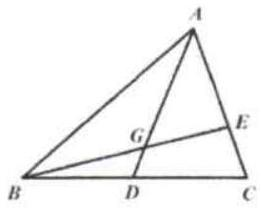
\includegraphics[width=\textwidth]{images/106(3).jpg}
\end{center}

Draw \(D F / / B E\) through and meets \(A C\) at \(F\). Since \(D\) is the midpoint of \(B C, F\) is the midpoint of \(E C\). Since \(A C=3 C E, A E\) \(=2 C E=4 E F\).\\
We also know that \(D F / / B E\). So \(A G: G D=A E: E F=4: 1\).\\
\centering
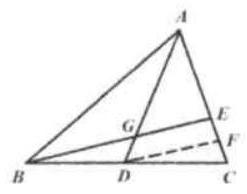
\includegraphics[width=\textwidth]{images/106(2).jpg}


\end{document}
